% !TeX encoding = utf8
% !TeX spellcheck = fr

\chapter{Circuits}\label{cha:tasks}

\xc{} fournit un système complet de fonctionnalités de gestion des circuits sur la campagne. Ils peuvent être
édités avant le décollage et, lors d'un vol d'agrément
sur la campagne, être modifiés en vol. Le passage au point de virage suivant est automatique,
mais peut aussi être effectué manuellement. Beaucoup des calculs d'\xc{} sont en lien avec
soit les points de virages, soit le point d'arrivée.
À moins qu'un ``vrai'' circuit ne soit défini, \xc{} fournira une fonction ``Retour au point de départ'',
sachant que beaucoup des fonctionnalités liées aux circuits font référence au lieu de décollage.
Ce chapitre décrit aussi l'utilisation d'enregistreurs IGC avec \xc.

Il y a trois modes de circuit~:
\begin{description}
\item[Circuit prévu] C'est le mode de circuit normal,
dans lequel le circuit est constitué d'un point de départ, de zéro ou plus point de virage
et d'un point d'arrivée. Les points doivent être passés dans un ordre défini.
\item[Circuit ``Aller à''] Vol vers un point unique.
\item[Dégagements] Fournit des propositions de vol vers les  terrains posables les plus proches.
\end{description}

Notez qu'en mode ``Aller à'' ou ``Dégagements'', le circuit prévu est conservé et peut être repris plus tard.
Les statistiques relatifs à un circuit accompli sont conservées.

\subsection*{Circuit ``Aller à'' automatique}

Si aucun circuit prévu n'est actif, alors, au moment du décollage, un circuit ``Aller à'' est automatiquement
créé et activé avec pour point d'arrivée le point de décollage ou l'aérodrome le plus proche
s'il est voisin du point de décollage.

Qu'un circuit soit défini ou pas, le point de décollage est toujours
créé et est affiché dans la liste des points de virage comme référence ou pour une utilisation ultérieure.

Après qu'un circuit prévu ait été défini pour la première fois, la fonction automatique ``Aller au point de décollage''
est désactivée. Pour faire un circuit simple, utiliser ``Aller à''.

\section{Circuits ``Aller à''}

Un circuit ``Aller à'' peut être défini simplement en sélectionnant un point de virage sur la carte
dans la liste des points de virage ou un autre moyen, comme en ouvrant le fenêtre de dialogue sur les dégagements
et en y sélectionnant \bmenuw{Aller à}. En mode circuit ``Aller à'', sélectionner
\bmenug{Nav. 2}\blink\bmenug{Circuit Reprendre}
permet de reprendre le circuit prévu (s’il y en avait un).

\section{Édition des circuits}

Plusieurs méthodes sont possibles pour éditer des circuits. Certaines sont plus efficaces au sol lors
de la préparation du circuit, d'autres sont utiles pour modifier le circuit en vol lors
de vols d'agrément sur la campagne. Les circuits peuvent être sauvegardés dans
un fichier pour être utilisés plus tard ou transférer entre différents plateformes \xc{}
(Android, Windows, Linux\textellipsis).

\tip{} Il est aussi possible d'enregistrer un circuit ``par défaut'' et être ensuite rechargée
automatiquement lors du démarrage du \xc. Une utilisation de cette fonction est de
configurer un circuit par défaut avec comme unique point de virage votre aérodrome --- cela signifie
qu'\xc{} est alors programmé par défaut pour une arrivée finale en finesse vers votre aérodrome de départ, ce qui
est utile pour des vols d'agrément sur la campagne.

Les principales méthodes de définition des circuits sont~:
\begin{itemize}
\item utilisation de la fenêtre d'édition de circuit.
\item Sélection de points de virage sur la carte, avec ajout au circuit en utilisant la fenêtre ``Détails''.
\item Charger le circuit à partir d'un fichier.
\end{itemize}


Le chargement d'un circuit à partir d'un fichier peut-être très utile en compétition ou pour ceux 
qui font un même circuit à plusieurs, une seule personne le 
distribuant aux autres, permettant ainsi de ne pas avoir à créer plusieurs fois le même circuit.
\tip{}
Si aucun circuit n'est présent au démarrage, un circuit est créé automatiquement.
Il contient un unique point de virage qui est le lieu de décollage et est utilisé par la fonction ``Aller au point de décollage''.

\xc{} sauvegarde le circuit en cours quand le programme est arrêté. A la mise en route,
le circuit est rechargé. Ceci permet de préparer un circuit tôt dans la journée et d'éteindre l'appareil sur lequel \xc{} fonctionne
et de le remettre sous tension juste avant le décollage.

Les points de virage des circuits sont sauvegardés même si le fichier de
points de virage est modifié. Ce qui veut dire que si vous sauvegardez un circuit puis changez le
fichier de points de virage, alors rechargez à nouveau le circuit, de nouveaux points de virage seront créés
pour chaque point de virage manquant dans le nouveau fichier.

\section{Informations sur les points de virage}

La page des détails des points de virage décrit en détail un point de virage et possède
des fonctionnalités de navigation comme ``Aller à'', ``Insérer dans le circuit'', ``Ajouter au circuit'' et ``Définir comme nouveau point de départ''.

On peut accéder de différentes façons aux informations sur les points de virage~:
\begin{itemize}
\item
\gesturespec{rd} le menu~\bmenug{Nav. 1}\blink\bmenug{Circuit},
en sélectionnant un des points de virage du circuit en cours, appuyer dessus une seconde fois pour faire apparaître la fenêtre de gestion des points de virage, puis utiliser le bouton  \bmenug{Détails}.

\item
\gesturespec{dl} le \bmenug{Nav. 1}\blink\bmenug{Dégagmts} 
pour afficher les
détails des terrains posables les plus proches.

\item
\gesturespec{dr} le menu \bmenug{Nav. 1}\blink\bmenug{Liste des waypoints}, puis surligné un point de virage
et \bmenuw{Sélectionner} un point de virage.

\item
\gesturespec{urdl} le menu \bmenug{Affich. 1}\blink\bmenug{Panor. On} pour afficher la
carte en mode panorama, puis aller jusqu'au point de virage recherché et toucher son étiquette ou son
symbole.

\item
\gesturespec{urdl}  le menu \bmenug{Info. 1}\blink\bmenug{Qu'y a-t-il ici~?}
pour afficher la
liste des éléments qui se trouvent sous le curseur ou sous votre doigt sur la carte.

\end{itemize}

\subsection*{Détails des points de virage}\label{sec:waypointdetails}
Cette fenêtre donne des informations sur un point de virage~: nom du point de virage,
coordonnées GPS, altitude, fréquence radio et l'axe de piste et sa longueur (si ces informations sont dans le fichier de points de virage),
heures locales de lever et de coucher du soleil, cap et distance, hauteurs nécessaires
pour atteindre ce point (voir détails ci-dessous). De plus, il y a aussi un bouton
\button{Aller à} qui permet de démarrer directement
une navigation vers ce point. L'utilisation de ce bouton annule le circuit en cours.
\begin{center}
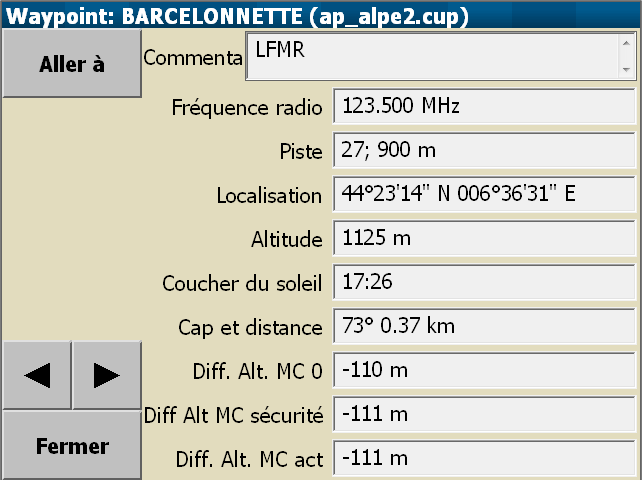
\includegraphics[angle=0,width=0.8\linewidth,keepaspectratio='true']{figures/dialog-waypointdetails0.png}
\end{center}

Comme mentionné ci-dessus, cette fenêtre affiche aussi trois types de différences d'altitude pour le point de virage considéré
(c'est-à-dire de hauteur nécessaire pour atteindre le point de virage à la hauteur de sécurité)~:
\begin{description}
\item[Diff. Alt. MC 0] Différence d'altitude avec un calage MacCready à zéro.
\item[Diff Alt MC sécurité] Différence d'altitude avec le calage MacCready de 
sécurité (voir~\ref{sec:secu-parameter}).
\item[Diff. Alt. MC act.] Différence d'altitude au calage MacCready actuel.
\end{description}

La fenêtre des détails des points de virage est constituée de deux pages, accessibles avec les touches
\bmenuw{$>$} et \bmenuw{$<$} situées au coin inférieur gauche.
En fonction de l'existence et du nombre d'autres détails propres au point de virage visualisé,
d'autres pages pourront être disponibles.

\subsection*{Points de virage et circuit}
La deuxième page des ``Détails de points de virage''
comporte une colonne de boutons permettant plusieurs actions concernant le point de virage sélectionné~:
\begin{description}
\item[\button{Remplacer dans le circuit}] Remplace le point de virage actif du circuit en cours par le point de virage sélectionné.
\item[\button{Insérer dans le circuit}] Insère le point de virage sélectionné avant le point de virage actif du circuit en cours.
\item[\button{Ajouter au circuit}] Ajoute le point de virage sélectionné à la fin du circuit en cours.
\item[\button{Retirer du circuit}] Retire le point de virage sélectionné du circuit en cours. Cette option est visible seulement si le point de virage sélectionné fait partie du circuit en cours.
\item[\button{Définir comme nouveau point de départ}] Définit le point de virage sélectionné comme nouvelle base de départ.
\item[\button{Afficher le point de virage}] Passe en mode panorama et se centre sur le point de virage sélectionné
\item[\button{Sélectionner la fréquence active}] %TODO à définir
\item[\button{Sélectionner la fréquence Standby}] %TODO à définir
\item[\button{Editer}] Permet de modifier les différents attributs du point de virage sélectionné
\end{description}

C'est une bonne habitude que de définir votre point ``Base'' à partir de cette fenêtre de détails
des points de virage. \xc{} démarre avec ce point comme base de départ même s'il
n'y a pas de signal GPS.\@ Quand aucune base n'est définie, la base par défaut est le centre de la carte.

\subsection*{Informations Aérodromes}
Cette page peut contenir des informations pertinentes
extraites des documents aéronautiques
à propos de l'aérodrome, dont les pistes, les fréquences radios, les circuits d'approche, les contacts.
Voir paragraphe~\ref{sec:Airfield-details}.
\begin{center}
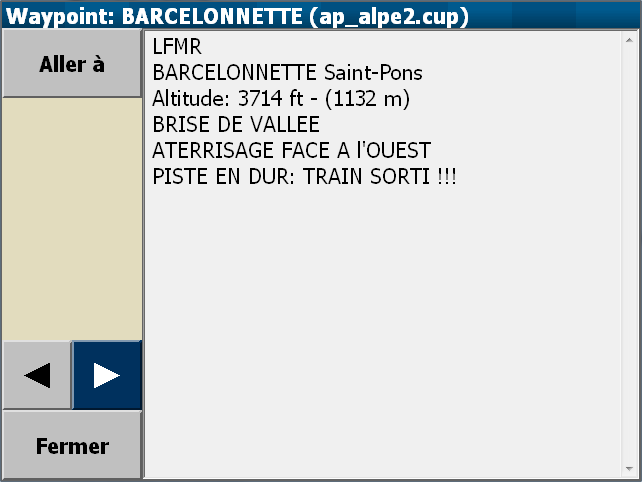
\includegraphics[angle=0,width=0.8\linewidth,keepaspectratio='true']{figures/dialog-waypointdetails1.png}
\end{center}

\subsection*{Image de détails du point de virage}
Cette page affiche une image satellite du point de virage.

\begin{center}
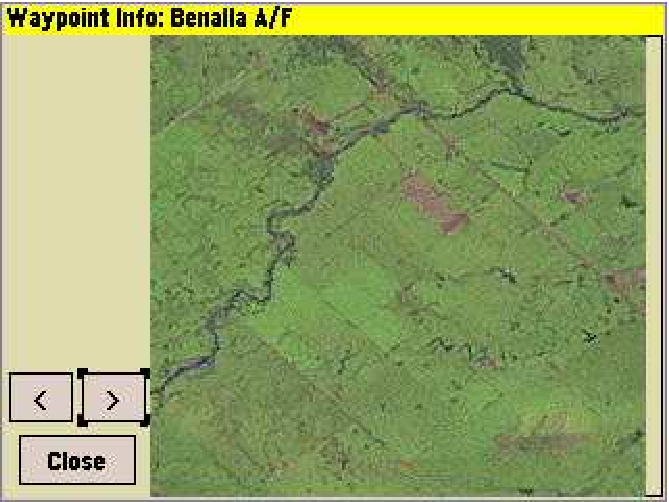
\includegraphics[angle=0,width=0.8\linewidth,keepaspectratio='true']{figures/dialog-waypointdetails2.pdf}
\end{center}
Pour savoir comment configurer les informations détaillées des points de virage, allez au paragraphe~\ref{sec:airfield-details}.

\section{Sélection des points de virage}\label{sec:waypoint-selector-dialog}

La fenêtre de sélection des points de virage permet de retrouver facilement
un point de virage dans une liste pouvant être très longue. \gesturespec{dr}

Le sélecteur de point de virage propose une fonction de filtrage avec une série de
\menulabelr{\bmenug{Nav 1/2}\blink\bmenug{Liste des waypoints}}
filtres optionnels sur le coté gauche de la page et, sur la droite, une liste des points de virage correspondants.
Plusieurs filtres sont disponibles. Ils peuvent être combinés, utilisés individuellement, voire pas du tout.
\begin{description}
\item[Nom] Tri basé sur les premières lettres du nom du point recherché. Au fur et à mesure que les caractères du nom sont choisis, la liste affichée se réduit pour faciliter la sélection.
\item[Distance] Affichage des points de virage se trouvant à l'intérieur d'un cercle, centré sur le planeur, dont on définit le rayon.
\item[Direction] Affichage des points de virage qui sont dans un cap défini par rapport au planeur.
Une direction spéciale ``HDG(xx°)'' (``HDG'' pour ``heading'', c.-à-d. ``cap'')
 montre les points de virage qui sont dans les 30° de part et d'autre de la route du planeur (ici route au 125). Ceci permet au pilote de répertorier rapidement les points de virage se trouvant dans la direction qu'il suit.
\item[Type] Affiche les points de virage qui sont du type choisi (posable, aérodrome, point de virage, etc.)
ou qui sont dans le fichier principal de points de virage ou dans le fichier secondaire
ou parmi ceux récemment utilisés.
\end{description}
Quand on trie par nom et par type, le résultat est classé par ordre alphabétique des noms. Quand (en plus) on tri par distance ou par direction, le résultat est classé par distance.

\begin{center}
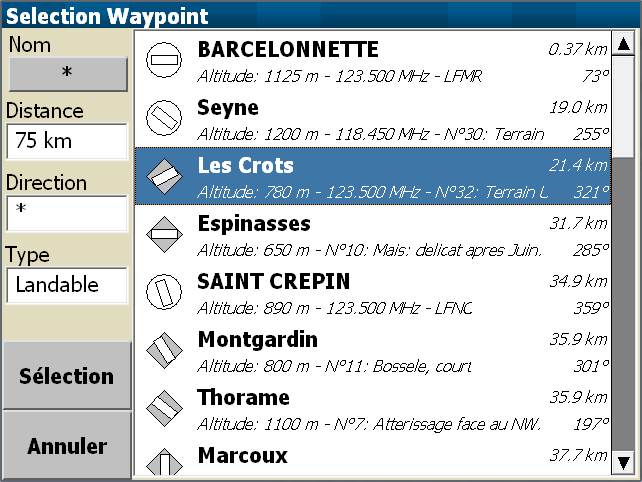
\includegraphics[angle=0,width=0.8\linewidth,keepaspectratio='true']{figures/dialog-waypointselect.png}
\end{center}

Si la liste de résultats est longue, on peut la faire descendre ou monter à l'aide de l'ascenseur de droite. 

La sélection d'un des éléments de la liste conduit à un comportement différent suivant la fonctionnalité qui à été utilisée précédemment. Le cas le plus courant est l'ouverture de la fenêtre de détails du point sélectionné. 

\section{Gestionnaire de circuits}\label{sec:task-manager-dialog}
\gesturespec{rd}

Le gestionnaire de circuits permet d'éditer, de voir, de charger, de modifier, de sauvegarder dans un fichier et de déclarer les circuits.
\menulabelr{\bmenug{Nav. 1/2}\blink\bmenug{Circuit}}

La première page du gestionnaire de circuit montre divers calculs
relatifs au circuit en cours, comme expliqué en détails après. De plus, il y a 
des boutons pour ouvrir les onglets
\bmenuw{Points de virage}, \bmenuw{Gérer},
and \bmenuw{Règles}, ainsi qu'un bouton pour \bmenuw{Fermer} le gestionnaire de circuits.

\subsection*{Calculateur de circuit}\label{sec:task-calc-dial}
La fenêtre du calculateur de circuit permet au pilote de voir l'effet de
différents modifications du circuit sur la performance finale.
\menulabelr{\bmenuw{Calc.\ circuit}}

En vol, le calculateur de circuit peut aussi être atteint par les pages d'analyses.
Dans les pages Circuit, Vario.\ et Vitesse circuit, un bouton \bmenuw{Calc.\ circuit} s'affiche,
et permet d'accéder directement à la fenêtre du calculateur de circuit.

\begin{center}
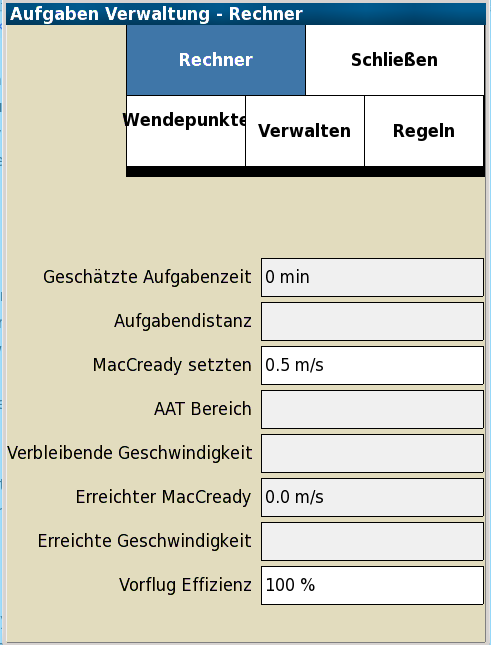
\includegraphics[angle=0,width=0.8\linewidth,keepaspectratio='true']{figures/dialog-taskcalculator.png}
\end{center}

\begin{description}
\item[Durée circuit estimée] Ce champ affiche la durée totale estimée
du circuit en le terminant avec le calage MacCready choisi.
\item[Durée restante] %TODO: To define
\item[Distance circuit] Ce champ affiche la distance totale du circuit.
\item[Distance restante] Ce champ affiche la distance restante pour terminer le circuit.
\item[Vitesse estimée] Ce champ affiche la vitesse estimée pour le
reste du circuit considérant le calage MacCready choisi.
\item[Vitesse Moyenne] %TODO: To define
\item[Entrer MacCready] Permet au pilote de faire varier le calage MacCready et d'observer son influence sur la durée estimée du circuit.
\item[Distance AAT] Permet à l'utilisateur d'ajuster les objectifs dans les zones AAT
restantes, pour voir l'effet que cela a sur la durée estimée du circuit et la longueur du circuit.
\item[Vitesse restante]
\item[MacCready réalisé] Ce champ affiche la valeur MacCready réalisée.
\item[Vitesse réalisée] Ce champ affiche la vitesse réalisée %TODO at the achieved MacCready setting???
\item[Efficacité en transition] 100~\% indique une performance égale au calage MacCready. Plus de 100~\% indique une performance supérieure à celle du calage MacCready (ex.~: sous des rues de nuage)~; et moins de 100~\% si vous êtes souvent à côtés de vos pompes.
Cet indice évalue la performance du vol en croisière en fonction de l'historique du vol avec le calage MacCready choisi.
Les calculs démarrent à partir du passage de la ligne de départ.
\end{description}
Pour plus de détails sur les calculs de la vitesse du circuit et les MacCready réalisés, allez au paragraphe~\ref{sec:task-speed-estim}.

Lors de la fermeture de la fenêtre, la valeur du MacCready entrée est utilisée comme calage du
MacCready pour les calculs. Si le bouton \bmenuw{Annuler} est enfoncé, le calage MacCready n'est pas modifié.

Pour les circuits AAT, le bouton \bmenuw{Objectif} ajuste la distance
(à la hausse ou à la baisse) de sorte que la durée estimée du circuit soit supérieure de moins de cinq minutes à la durée impartie du circuit. La distance est ajustée en fonction
des points objectifs restants. Habituellement, tous les objectifs sont réglés sur ``Optimisé'', ce qui fait que le pilote
n'a pas à s'occuper de repositionner manuellement les points objectifs pour trouver la meilleure distance à parcourir dans le temps imparti, diminuant ainsi la charge de travail du pilote.

\subsection*{Points de virage}
L'onglet \button{Pts de virage} affiche une liste ordonnée des points de virages du circuit en cours.
\menulabelr{\bmenuw{Pts de virage}}
S'il n'y a pas de point de virage dans le circuit, seul
``Ajouter point de virage'' est affiché.
En sélectionnant ce menu, le sélecteur de points de virage apparaît
comme décrit précédemment. Appuyez deux fois sur un point de virage de la liste ajoute ce point de virage au circuit.


\subsection*{Gérer}
Cet onglet permet d'accéder à toutes les opérations nécessaires pour créer de nouveaux circuits ou gérer
\menulabelr{\bmenuw{Gestion}}les circuits déjà existants.
Quatre boutons peuvent être sélectionnés~:
\begin{itemize}
\item [\bmenuw{Nouveau circuit}] Efface le circuit courant de la mémoire de travail et rétablit 
les règles par défaut.
\item [\bmenuw{Déclarer}] Si un enregistreur externe est connecté, ceci permet de
charger le circuit actif vers l'enregistreur et de le déclarer.
\item [\bmenuw{Circuits enregistrés}] Affiche la liste des circuits enregistrés, permettant au pilote de charger un circuit précédemment enregistré. Notez que cette action écrasera le circuit
en cours.
\item [\bmenuw{Enregistrer}]  Sauvegarde le circuit actif courant.
En appuyant sur \bmenuw{Enregistrer} un nom de fichier vous sera demandé.
\end{itemize}

\subsection*{Règles}
Les champs affichés en appuyant sur \menulabelr{\bmenuw{Règles}} 
dépendent du type de circuit choisi. En sélectionnant un champ,
une fenêtre apparaît pour permettre de modifier
la valeur de cette règle. Les types de circuit sont expliqués en
détails juste après.

De plus, en appuyant de nouveau sur le bouton \bmenuw{Règles} après qu'il eut déjà été sélectionné permet
de basculer entre une vue miniature de la carte du circuit et une vue plus grande du circuit.

\section{Types de circuit}
\xc{} permet actuellement de définir trois différents types de circuits~: course, AAT et insignes/records FAI.\@

Une description sommaire de ces types de circuit est donnée ci-dessous. Cependant ce manuel
ne paraphrase pas les règles FAI ou celles des types de circuit de concours. Le
lecteur est encouragé à connaître parfaitement chaque type de circuit en se référant aux règles des compétitions
et aux règles FAI.\@ Les règles FAI sont disponibles sur \url{http://www.fai.org}. 

\subsection*{Course (course sur circuit)}
Une course sur circuit implique un passage obligatoire à chaque point de virage défini et dans l'ordre fixé. 
Le choix de ce type d'épreuve permet de définir les valeurs des champs suivants
(note~: si l'option ``Règles de départ/arrivée FAI'' est mise à ``On'', alors seule une partie de ces options est disponible)~:
  \begin{description}
  \item [Arme départ manuellement] Si mis sur ``On'', des boutons supplémentaires seront dans le menu \bmenug{Nav. 1/2} afin de vous permettre d'\bmenug{Armer le départ} et de \bmenug{Désarmer le départ}, contrôlant ainsi la détection de la condition de départ.
  \item [Heure d'ouverture du départ] L'heure à laquelle la zone de départ ouvre.
  \item [Heure de fermeture du départ] L'heure à laquelle la zone de départ ferme.
  \item [Vitesse max.\ au départ] La vitesse maximale autorisée dans la zone d'observation et au passage de la ligne de départ.
  Si la vitesse n'est pas limitée, il faut mettre 0~km/h.
  \item [Hauteur max.\ départ] La hauteur maximale autorisée dans la zone d'observation et au passage de la ligne de départ.
  C'est une hauteur maximale autorisée pour l'épreuve au-dessus de la hauteur de référence (AGL ou MSL). S'il n'y a pas de limite, il faut mettre 0~m.
  \item [Réf.\ hauteur départ] Définit la référence pour la hauteur maximale du point de départ~: au-dessus du sol (``AGL'') ou bien au-dessus du niveau moyen de la mer (``MSL'').
  \item [Hauteur min.\ arrivée] La hauteur minimale de passage au-dessus de la ligne d'arrivée. 
  C'est une hauteur minimale autorisée pour l'épreuve au-dessus de la hauteur de référence (AGL ou MSL). S'il n'y a pas de limite, il faut mettre 0~m.
  \item [Ref.\ hauteur arrivée] Définit la référence pour la hauteur minimale du point d'arrivée~: au-dessus du sol (``AGL'') ou bien au-dessus du niveau moyen de la mer (``MSL'').
  \end{description}

\subsection*{AAT (épreuve de vitesse sur secteurs) et MAT (circuit à secteurs modifiés)}
C'est un circuit passant par des zones définies (cylindres ou secteurs) qui doit être effectué sur une durée minimale imposée.
Le choix de ce type d'épreuve permet de définir, en plus des champs définis pour un circuit de type ``Course'' (voir ci-dessus) la valeur du champ suivant~:
  \begin{description}
  \item [Durée mini AAT] Durée minimum requise pour l'épreuve.
  Se référer aux documents officiels pour plus de détails, surtout pour le calcul des pénalités lors de l'arrivée avant la durée minimum impartie.
 \end{description}

\subsection*{Insignes/records FAI}
Le choix de ce type d'épreuve permet de définir la valeur du champ suivant~: 
  \begin{description}
  \item [Règles de départ/arrivée FAI] Si mis sur ``On'', seuls le mode d'armement et les heures d'ouverture et de fermeture du départ peuvent être paramétrés.
Si mis sur `Off'', toutes les autres règles de circuits peuvent être modifiées par rapport au FAI normal (voir ci-dessus le type de circuit ``Course''). 
  \end{description}

Quand le type de circuit a été choisi et que les règles de départ et d'arrivée
ont été définies comme décrit ci-dessus, il faut préciser les propriétés
de chaque point de virage du circuit.

Une fois sélectionnés, les points de virage peuvent être déplacés avec les flèches Haut et Bas.
Le premier point de virage est automatiquement un point de type ``Départ'' et le dernier un point de type ``Arrivée''.

\section{Règle de circuit pour les points de virage}\label{sec:task-rules}

La fenêtre de \bmenuw{points de virage} montre la liste des points de virage du circuit.
\menulabelr{\bmenuw{Points de virage}} Si aucun point n'est encore défini, cette fenêtre
affichera une liste vide. Avec \bmenuw{(Ajouter point de virage)}, flèches Haut et Bas, et
\bmenuw{Pt d'arrivée}, une liste ordonnée de points de virage est créée.
Un point de virage peut être un point de départ, un point de virage ou un point d'arrivée.
En appuyant 2~fois sur le point de virage désiré (ou une fois puis sur \button{Éditer le point}) ouvre la fenêtre d'édition des points de virage.
En appuyant sur \button{Modifier le type} on obtient la liste des différents types de point de virage possibles.
Un rappel de la définition du point et de sa spécificité est affiché en bas de la liste.

Différentes règles de circuit peuvent être utilisées lors de la définition d'un circuit, dont les triangles FAI habituels et les AAT.\@
De nombreux détails des règles peuvent être configurés.

Les lignes de départ et d'arrivée sont centrées sur le point de virage associé
et sont alignées perpendiculairement au point de virage suivant ou précédent,
selon le cas.

Les secteurs de points de virage
sont des quadrants de 90~degrés alignés sur la bissectrice des
points de virage précédent et suivant, comme il est d'usage dans les circuits FAI.\@
Il est aussi possible de définir des secteurs britanniques (BGA) et allemands (DAeC).

\subsection*{Types de point de départ}
Les conditions de validité du départ dépendent du type de départ~:
\begin{description}
\item[Cylindre de départ] Quand le planeur quitte la surface du cylindre.
\item[Ligne de départ] Quand le planeur passe la ligne en direction du premier point de virage.
\end{description}

\subsection*{Types de point de virage}
Les conditions de validité de passage aux points de virage intermédiaires dépendent de leur type~:
\begin{description}
\item[Quadrant FAI] Passage dans la zone définie par un quart de cercle de 20~km de rayon, centré sur le point de virage et orienté sur la bissectrice de l'angle.
\item[Secteur en trou à clef (secteur DAeC 0,5/10)] Règles allemandes.
Passage dans un secteur de 90° centré sur la bissectrice de l'angle et de 10~km de rayon.
Le secteur inclue aussi un cylindre de 500~m de rayon.
\item[Épreuve de type BGA]  Règles britanniques. Passage dans un secteur de 90° centré sur la bissectrice de l'angle et de 20~km de rayon.
Le secteur inclue aussi un cylindre de 500~m de rayon.
\item[Épreuve de type BGA avec option] Règles britanniques. Passage dans un secteur de 180° centré sur la bissectrice de l'angle et de 10~km de rayon.
Le secteur inclue aussi un cylindre de 500~m de rayon.
\item[Cylindre de point de virage]  Passage dans un cylindre centré sur le point de virage.
\item[Quadrant symétrique] Un quadrant symétrique d'un rayon configurable.
\item[Zone secteur de cylindre (AAT)]  Passage dans un cercle, ou portion de cercle, centré sur le point de virage.
\item[Zone secteur de couronne (AAT)]  Passage valable si dans une couronne, ou portion de couronne, centré sur le point de virage.
\end{description}

\subsection*{Types de point d'arrivée}
La validité du passage du point d'arrivée dépend de son type~:
\begin{description}
\item[Quadrant d'arrivée FAI] Un secteur de 90~degrés d'un rayon de un kilomètre. Traverser le bord pour terminer le circuit.
\item[Ligne d'arrivée] Quand le planeur passe la ligne en direction opposée au dernier point de virage.
\item[Cylindre d'arrivée] Quand le planeur entre dans la surface du cylindre.
\end{description}

L'avancée automatique au point suivant est effectuée dès qu'une des conditions est remplie. Pour démarrer un AAT, un circuit mixte, ou un circuit de course, le départ doit être préalablement armé.

\tip{} Les règles de compétition peuvent être définies dans un fichier de profil et distribuées au groupe de pilotes ou personnes définissant les circuits afin qu'ils puissent concourir avec les mêmes règles~!

Des règles supplémentaires pour les points de départ et d'arrivée peuvent aussi être définies~:  pour les départs, une hauteur maximale au-dessus du sol et une vitesse maximale~; pour les arrivées, une hauteur minimale au-dessus du sol. Ces paramètres sont modifiables dans le menu\config{taskrules} \bmenug{Config. 1/3}\blink\bmenug{Système} dans les onglets ``Circuit/Règles'' et ``Circuit/Types de point de virage''.
Pour les circuits qui ne sont pas des AAT, une option est disponible afin de paramétrer l'altitude minimum d'arrivée, en accord avec les règles FAI.\@ Dans ce cas, l'altitude d'arrivée doit être inférieure de moins de 1000 mètres à celle du départ.

\section{Démarrage du circuit}\label{sec:start-task}
Une fois que les points de virage (départ, points de virage et leur particularités, arrivée) ainsi que les règles du circuit sont bien définis, il reste deux choses à faire~:
\begin{itemize}
\item Dans l'onglet ``Gérer'', appuyer sur \button{Enregistrer} pour sauvegarder le circuit en lui donnant un nom, ou si vous venez de modifier un circuit existant, lui donner le même nom ou un autre nom si vous souhaitez en créer un nouveau à partir de celui préexistant.
\item Appuyer sur le bouton \button{Fermer} du gestionnaire de circuit.
Suivant les créations et modifications faites auparavant, les fenêtres qui apparaissent sont différentes.
Vous pouvez choisir \button{Fermer} pour utiliser le circuit que vous venez de modifier ou de créer.
Le bouton \button{Annuler les modifications} permet d'oublier les modifications faites et de continuer avec le circuit qui était chargé précédemment.
Si vous avez créé un nouveau circuit et que vous l'avez enregistré, il n'est pas perdu~: vous le retrouverez plus tard dans la liste des circuits enregistrés.
Par contre le circuit qui était en cours, lui, a bien été effacé de la mémoire de travail.
Il vous faut donc recharger le circuit que vous souhaitez réaliser.
\end{itemize}
Si vous avez appuyé sur \button{Fermer}, le circuit est démarré (actif).

\section{Déroulement et faux départs}\label{sec:advanc-rest-tasks}
À chaque instant un point de virage du circuit est désigné comme point de virage
actif. Le point de virage actif est utilisé pour les calculs et l'affichage des
informations de navigation (aussi nommé ``Point de virage suivant'' dans la
description des InfoBoxes du chapitre~\ref{cha:infobox}).

En vol, la direction à suivre pour atteindre le point actif est affichée en permanence.

L'altitude requise pour terminer le circuit est calculée pour la trajectoire partant
de la position présente du planeur, passant par tous les points de virage et allant
jusqu'au point d'arrivée.

Le passage au point de virage suivant est automatique ou manuel.
Le point de départ d'un circuit en compétition, ainsi que les points des circuits AAT, sont particuliers et nécessitent
que le point du circuit soit ``armé'' avant que le système n'avance automatiquement au prochain point du circuit une fois que ce point a été passé.

Pour les circuits hors-compétition, aucune interaction avec l'utilisateur n'est nécessaire pour
changer de point sur le circuit --- le système avancera automatiquement lorsque
chaque point sera atteint. L'utilisateur peut toujours sélectionner manuellement le point suivant ou revenir au point
précédent en sélectionnant soit le menu \bmenug{Nav. 1/2}\blink\bmenug{Point de virage précédent}, soit le menu \bmenug{Nav. 1/2}\blink\bmenug{Point de virage suivant}.

Les boutons \bmenug{Point de virage précédent} et \bmenug{Point de virage suivant}
affichent des étiquettes dynamiques indiquant l'action qui sera faite si l'on appuie dessus.

Pour les points de virage nécessitant d'être armé, \bmenug{Point de virage suivant} devient 
\bmenug{Armer le virage} si le point de virage n'est pas armé et,
s'il est armé,
\bmenug{Point de virage suivant}, permettant l'avance manuelle.
\bmenug{Point de virage précédent} devient \bmenug{Désarmer le virage} si le point de virage est armé,
et vice-versa. De même, pour les circuits de compétition, ces menus se mettent à jour pour armer
les points de départ. Si le point de virage suivant est le \bmenug{Point d'arrivée}, l'étiquette
du menu est adaptée en conséquence.


Des messages d'information apparaissent pour les points de virage nécessitant d'être armé une fois
dans la zone d'observation. Ce sont des rappels au pilote d'armer le point de virage quand il est prêt à passer au point de virage suivant. Pour le départ, une
alerte signale que le planeur est dans le cylindre de départ ou derrière la ligne de départ, afin de lui rappeler d'armer si nécessaire.

Pour les PC avec écran tactile, l'utilisateur peut
faire défiler manuellement d'un point à l'autre en sélectionnant le point de virage
 et en appuyant sur les touches Haut et Bas.

Voir le paragraphe~\ref{sec:task-rules} pour plus de détails concernant les règles des secteurs d'observation.

Si le pilote fait défiler les points de virage manuellement, cela ne signifie pas
que le planeur les a passé réellement~! Toutefois, cette
fonctionnalité est utile pour forcer un nouveau départ ou bien pour sauter un point de virage quand
on est sur un circuit d'agrément.

\tip{} Les circuits peuvent être redémarrés en faisant simplement défiler manuellement
les points de virage jusqu'au point de départ.

Dans tous les types de circuit, si le planeur rentre à nouveau dans la zone de départ ou bien repasse à 
nouveau la ligne de départ, le circuit est redémarré automatiquement.

En sélectionnant \button{Point de virage précédent} le système ``oubli'' que ce point
de virage a déjà été passé~: le gestionnaire de circuit
s'attend alors à devoir repasser par ce point de virage
avant de poursuivre le circuit. Le pilote peut toujours appuyer sur \button{Point de virage
suivant} pour sélectionner le prochain point de virage.

Un message associé à une alarme sonore apparaît à chaque passage au point de virage suivant. Les
messages sont affichés quand le système avance automatiquement au prochain point
de virage du circuit ou, en mode ``armé manuellement'', quand le système est armé et que le planeur est dans le secteur du point de virage~:
\begin{description}
\item[Démarrage circuit] apparaît au passage de la ligne de départ ou à la sortie du secteur de départ. Cela peut être fait plusieurs fois.
\item[Point de virage suivant] apparaît quand le planeur est entré dans le secteur
d'observation du point de virage. Les points de virage avec un objectif variable
sont passés dès l'appui sur le bouton \button{Armer point de virage}. En cas d'armement en mode manuel, si le
planeur est passé par le secteur d'observation et en est déjà sorti, appuyer sur ``armer'' suggérera
au gestionnaire de circuit que le pilote à l'intention de repasser
ce point de virage.
\item[Circuit terminé] apparaît lors du passage de la ligne
ou de l'entrée dans le cylindre d'arrivée. Cela survient en mode manuel comme en mode automatique.
\end{description}



\section{Points de départ multiples}\label{sec:alternate-starts}

Le gestionnaire de circuit permet de définir plusieurs secteurs de départ~:

\blink\bmenuw{Points de virage} sélectionne le point de départ, \menulabelr{\bmenug{Nav. 1/2}\blink
\bmenug{Circuit}}\bmenuw{Éditer le point}\blink\bmenuw{Ajout départs alternatifs}

Dans le gestionnaire de circuit, sur la page d'édition du point de départ, sélectionner le menu the \bmenuw{Activer départs alternatifs}. Un autre écran s'affiche pour définir un point de départ alternatif. Si des points de départs alternatifs
ont été définis précédemment, l'étiquette \bmenuw{Activer départs alternatifs} est transformée en \bmenuw{Modifier départs alternatifs}. Après avoir sélectionné ``Ajouter départs alternatifs''
et appuyer sur \bmenuw{Repositionner}, la fenêtre de filtrage ``Sélectionner point de virage'' s'affiche.

Ayant défini plusieurs points de départ alternatifs, la façon de faire avec ``prochain point de virage'' sera reproduite. Avant la détection d'un départ valide et l'ayant armé manuellement, les boutons faisant défiler tous les points de virage afficheront l'étiquette \bmenug{Prochain point de départ}.

En résumé, toutes les étiquettes dynamiques du menu \bmenug{Nav. 1/2} affiche des actions devant être
effectuées pour sélectionner les points de virage et leurs conditions, soit de manière consécutive, soit en ordre inversé.


\section{Abandon/reprise d'un circuit et dégagements}

Si les conditions atmosphériques se dégradent, le pilote peut juger que l'épreuve ne peut être terminée. Dans cette situation, \xc{} vous permet d'``abandonner'' le circuit~; il vous aidera
ensuite à atteindre un site d'atterrissage sûr. Un circuit peut être annulé de
différentes façons~: soit en sélectionnant un point de virage et en faisant un ``Aller à'', soit en sélectionnant ``Annuler''. Dans les deux cas, le circuit peut être repris.

\subsection*{Abandon de circuit}\label{sec:taskabort}
Passer en mode ``Abandon de circuit'' fait entrer \xc{} dans un cas spécial d'arrivée finale.
\menulabelr{\bmenug{Nav. 2/2}\blink\bmenug{Circuit Abandon}} Pour une discussion sur 
les modes de vol, aller au paragraphe~\ref{sec:flightmodes}. Dans ce mode de vol,
l'option de configuration ``Polaire pour zone d'atteinte'' permet de définir si
le calcul des hauteurs d'arrivée en mode abandon utilisent la valeur du MacCready avant
l'abandon du circuit ou la calage MacCready de sécurité. \config{reachpolar}
Par défaut, c'est la valeur de sécurité du MacCready qui est utilisée. Lors du passage en mode abandon, le calage MacCready est celui qui est le plus faible entre MacCready de sécurité et MacCready actuel.

Avec le passage en mode abandon, le circuit sur la campagne est ignoré. Sur la carte, des flèches
sont dessinées, pointant vers les terrains posables les plus proches,
assistant le pilote dans sa décision. Comme pendant le reste du vol, le groupe des terrains
posables proches est mis à jour en permanence. Les flèches et les plus proches terrains posables peuvent changer
dynamiquement en mode abandon, de telle façon qu'à chaque instant plusieurs options d'atterrissage soient 
proposées et peuvent être sélectionnées comme point de virage actif\sketch{figures/abort-low.png}. Même si aucun
terrain posable n'est à portée, les flèches sont dessinées.
\sketch{figures/abort-low.png} 
Si les conditions s'améliorent, le circuit peut être ``repris'' en sélectionnant le même
bouton que celui qui a annulé le circuit, maintenant nommé \bmenug{Circuit Reprendre}. Le point de virage
qui était actif avant l'abandon du circuit est alors réactivé, ainsi que tous les autres éléments du circuit.

\subsection*{Dégagements}\label{sec:alternates}
Les terrains de dégagements sont mis à jour tout au long du vol, ce qui permet un bonne conscience
de la situation en jetant un coup d'œil aux dégagements possibles.\menulabelr{\bmenug{Nav. 1/2}\blink
\bmenug{Dégagements}} Six options d'atterrissages
sont considérées. Elles sont filtrées par les critères de configuration de l'``ordre de dégagement''
(simple, circuit ou base). \config{alternatesmode}.
Choisir ``Circuit'' ou ``Base'' modifie l'ordre proposé des dégagements en favorisant 
la direction que vous aviez lorsque vous étiez encore en circuit.

Comme avec toute liste de points de virage, des informations supplémentaires peuvent être affichées en appuyant sur \bmenuw{Détails} avant de décider de son choix. Sélectionner le point de virage de la liste et appuyer sur \bmenuw{Aller à}.
\sketch{figures/alternates_list.png}

Bien que les éléments de la liste des dégagements suivent des règles différentes, ils ont le même comportement vis-à-vis du circuit en cours. Faire sa sélection dans la liste des dégagements annule le circuit en cours. Une fois que les conditions s'améliorent, la reprise du circuit en utilisant le bouton déjà mentionné.


\section{États du circuit}\label{sec:task-status}

Les fenêtres d'états donnent un aperçu des informations importantes sur le circuit en cours. 
\gesturespec{ldrdl} Elles sont utiles pour avoir une
vue générale des données du circuit et permettent de libérer des InfoBoxes pour afficher
d'autres paramètres. Les fenêtres d'état peut être consultées pour confirmer
qu'un départ valide a été détecté, mais aussi pour des informations sur le déroulement du circuit. 
\menulabelr{\bmenug{Info. 2/3}\blink\bmenug{États}}
Les fenêtres d'état peuvent être accédées par le menu ou en faisant un gauche-bas-droit-bas-gauche (un peu comme un S). Les onglets ``Circuit'' et ``Règles'' sont pertinentes.

L'onglet ``Circuit'' affiche en particulier la durée AAT, les distances parcourues et restantes, et les vitesses sur le circuit. 
L'onglet ``Règles'' donne en particulier la validité des points de départ et d'arrivée selon les règles du circuit.
\begin{center}
\begin{tabular}{c c}
Circuit & Règles \\
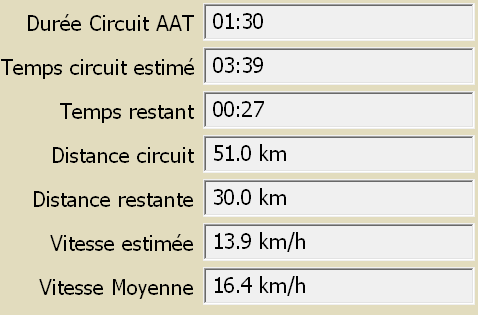
\includegraphics[angle=0,width=0.4\linewidth,keepaspectratio='true']{figures/status-task.png} &
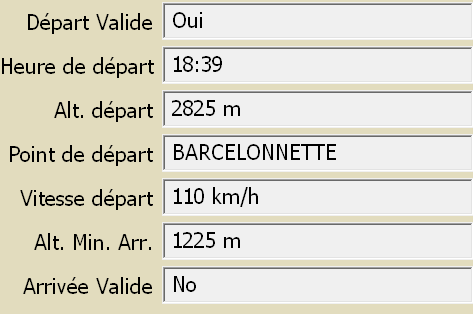
\includegraphics[angle=0,width=0.4\linewidth,keepaspectratio='true']{figures/status-rules.png} \\
\end{tabular}
\end{center}

\section{AAT (Assigned Area Tasks)}\label{sec:aat-tasks}

\subsection*{Objectifs AAT}

Un \emph{objectif} est un point dans une zone de virage AAT vers lequel le pilote
se dirige. Ces objectifs peuvent être déplacés à l'intérieur des zones AAT afin
que le pilote ajuste au mieux la distance du circuit. Les objectifs peuvent être positionnés
avant le vol, pendant la préparation du circuit et modifiés en cours d'épreuve.

Au cours d'un AAT, le calculateur dirige le planeur vers l'objectif.
Les statistiques comme la distance au point de virage sont calculées en se basant sur
l'objectif, et non sur la base du point de virage de la zone de l'AAT lui-même.

L'avance automatique au prochain point de virage n'est pas déclenchée directement
par l'entrée dans la zone AAT~: le pilote doit ``armer'' manuellement le passage au point de virage
suivant. En faisant cela, l'optimiseur de circuit est mis en route afin de relever
les coordonnées de l'objectif réalisé et de mettre à jour l'optimisation
de l'objectif pour le reste du circuit. Voir paragraphe~\ref{sec:advanc-rest-tasks} pour plus de détails.

\subsection*{Déplacement manuel des objectifs}

Dans le but de simplifier la définition des points objectifs, 
leur position est définie par un paramètre d'amplitude qui détermine à quelle
distance est l'objectif entre les distances minimale et maximale possibles.  
Il est exprimé comme un pourcentage. Par exemple, pour une amplitude de 100\%,
l'objectif est positionné pour avoir le plus grand circuit possible. Avec une amplitude de -100\%, l'objectif est positionné pour avoir le plus petit circuit possible. 

Une amplitude nulle donne un circuit de taille nominale~:
pour des secteurs, l'objectif est
à mi-distance le long du rayon de la bissectrice~; pour des cylindres, l'objectif est au
centre du cylindre.

La fenêtre de dialogue du calculateur de circuit (voir paragraphe~\ref{sec:task-calc-dial}) montre
le pourcentage moyen sur tous les points dans la gamme d'amplitude de l'AAT.\@
Les objectifs peuvent être modifiés un par un à partir de la fenêtre d'objectif du calculateur de circuit.

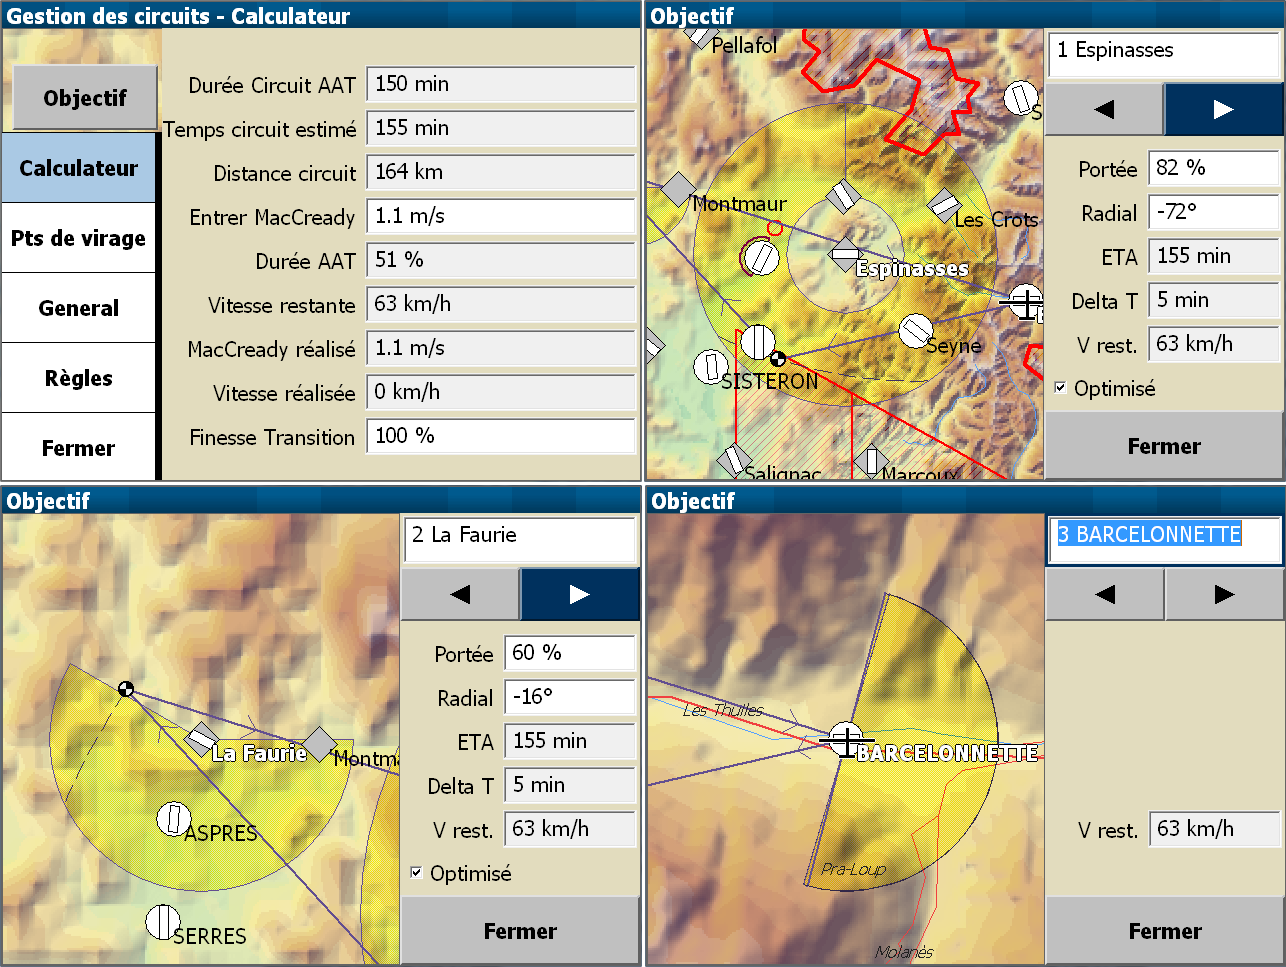
\includegraphics[angle=0,width=1.2\linewidth,keepaspectratio='true']{figures/gestion_circuit_00.png}



\subsection*{Objectifs AAT et calculateur de circuit}

Les objectifs lors d'une épreuve AAT sont typiquement utilisés comme ceci~:
\begin{itemize}
\item entrer les valeurs des paramètres MacCready, moucherons, ballast, force et direction du vent pour le vol en utilisant les fenêtres \menulabelr{\bmenug{Config. 1/3}\blink\bmenug{Vol}} et \menulabelr{\bmenug{Config. 1/3}\blink\bmenug{Vent}}.
\item Définir le circuit comme habituellement avec l'éditeur de circuits.
\item En se basant sur son expérience et son avis sur la météo du jour,
et si certaines zones sont probablement plus ou moins difficiles que
d'autres, les objectifs peuvent être définis individuellement pour chaque point de virage
dans la fenêtre d'objectif. Le paramètre ETA permet d'avoir une idée de la durée estimée du vol et de la comparer à
la durée impartie de l'épreuve. Le paramètre Delta~T permet de contrôler si le circuit
envisagé est efficace et suffisamment long.
\item En vol, si les conditions changent, comme l'adoption d'un autre calage MacCready ou une modification du vent estimé,
le gestionnaire de circuit peut être ouvert pour vérifier la durée estimée du vol, et de la comparer à la durée minimale.
\item Si le pilote décide d'allonger ou de raccourcir le circuit, tous les objectifs
restant peuvent être repositionnés à l'aide de le gestionnaire de circuit.
\end{itemize}

Le gestionnaire de circuit aide ainsi le pilote à répondre à la
question ``que se passera-t-il si~?'', telle que~:
\begin{itemize}
\item Que se passera-t-il si les conditions s'améliorent~? Le calage MacCready peut être
augmenté et le pilote peut voir s'il dispose d'assez de marge sur les objectifs pour
agrandir son circuit. 
\item Que se passera-t-il si les conditions se dégradent~? Le calage MacCready peut être
réduit et le pilote peut voir de combien le circuit peut être raccourci tout en
finissant le circuit après la durée minimale imposée.
\item Que se passe-t-il si je quitte la zone AAT maintenant~? En appuyant sur \button{Armer le
virage}, la prise en compte de la position actuelle par l'optimiseur de circuit est imposée. Le repositionnement des objectifs suivants peut être visualisé dans la fenêtre du gestionnaire de circuit.
\end{itemize}

\subsection*{Position de l'objectif}

\xc{} analyse en permanence le chemin du planeur dans les zones AAT pour calculer les points théoriques donnant le score maximum pour la distance parcourue effective. En interne, le programme déplace les objectifs des zones passées qui sont alors les objectifs optimaux. 

Dans certains cas l'objectif de la zone AAT active peut être déplacé automatiquement~:
\begin{itemize}
\item Quand à l'intérieur de la zone, l'objectif de cette zone est projeté sur la droite passant par l'objectif de la zone précédente et la position actuelle du planeur. Ceci permet au pilote de choisir d'entrer dans une zone AAT avec un autre cap ou avec un décalage par rapport à la ligne partant de l'objectif précédent et allant vers l'objectif actuel.

\item Quand le planeur est dans la zone AAT et que la distance à l'objectif précédent est supérieure à la distance au prochain objectif, l'objectif est alors projeté au devant du planeur sur la droite reliant le dernier objectif et la position actuelle du planeur. La trace n'est plus montrée mais la flèche bleue de direction optimale pointe dans la direction de cette droite.
\end{itemize}

A titre d'exemple, les figures suivantes illustrent comment le positionnement des objectifs évoluent au cours du vol et montrent comment \xc{} calcule le chemin théorique rapportant le plus de points.

\begin{maxipage}
\begin{center}
\begin{longtable}{|c|c|}
\toprule
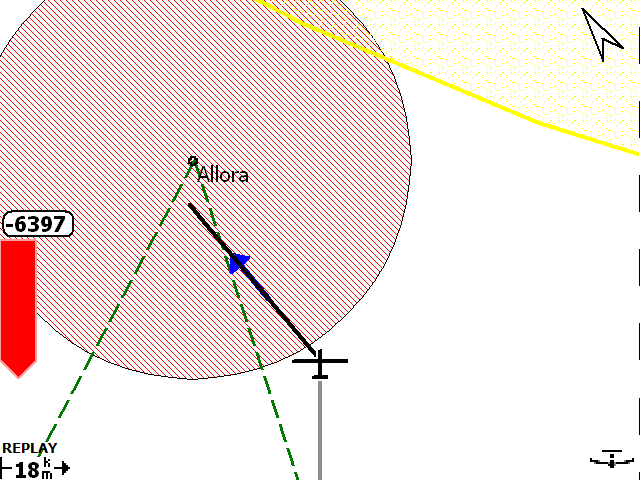
\includegraphics[angle=0,width=0.45\linewidth,keepaspectratio='true']{figures/faat01.png} & 
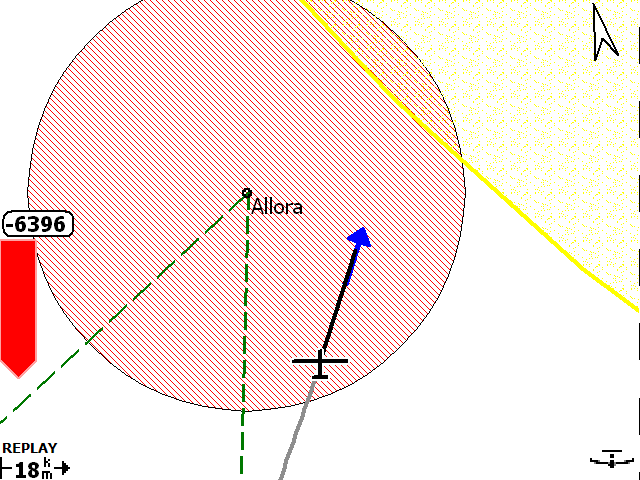
\includegraphics[angle=0,width=0.45\linewidth,keepaspectratio='true']{figures/faat02.png} \\
\emph{Hors zone} & \emph{Dans la zone} \\
Objectif (-20\%) sur la bissectrice & Objectif projeté sur la route \\

\midrule
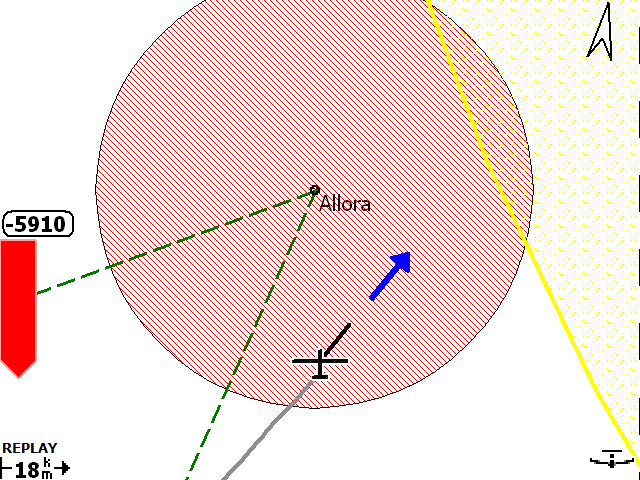
\includegraphics[angle=0,width=0.45\linewidth,keepaspectratio='true']{figures/faat03.png} & 
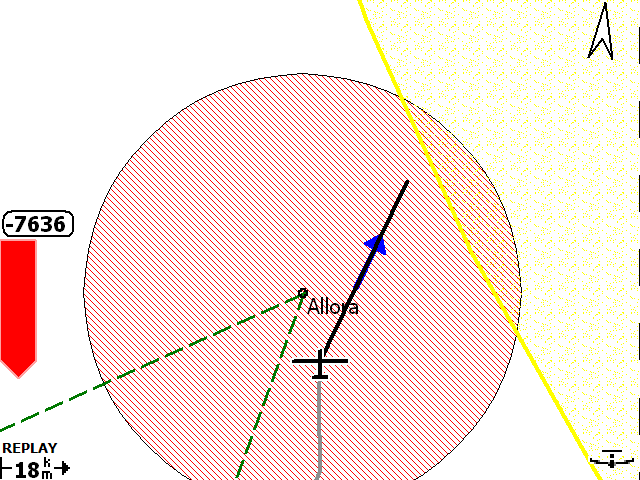
\includegraphics[angle=0,width=0.45\linewidth,keepaspectratio='true']{figures/faat04.png} \\
\emph{Distance AAT diminuée par le pilote} & \emph{Distance AAT augmentée par le pilote} \\
Objectif (-80\%) projeté sur la route & Objectif (80\%) projeté sur la route \\

\midrule
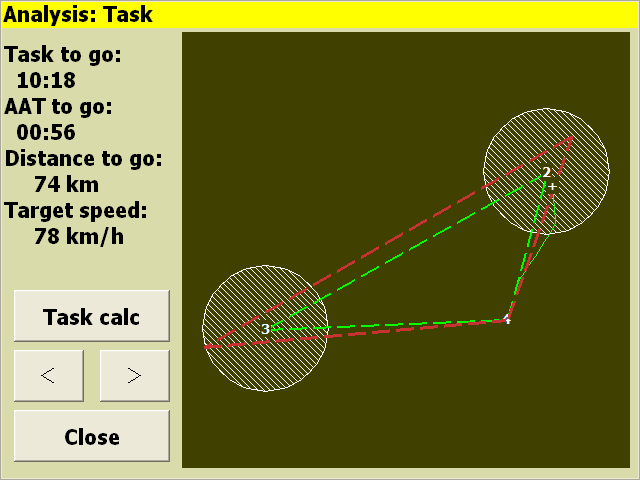
\includegraphics[angle=0,width=0.45\linewidth,keepaspectratio='true']{figures/faat05.png} & 
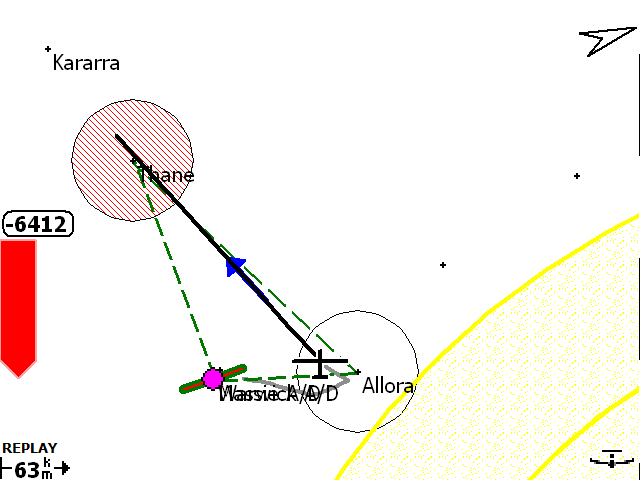
\includegraphics[angle=0,width=0.45\linewidth,keepaspectratio='true']{figures/faat06.png} \\
\emph{Analyses (page circuit)} & \emph{Prochain point de virage} \\
Chemin encadrant l'objectif actif & ``Armer virage'' appuyé \\
\bottomrule
\end{longtable}
\end{center}
\end{maxipage}

\begin{maxipage}
\begin{center}
\begin{longtable}{|c|c|}
\toprule
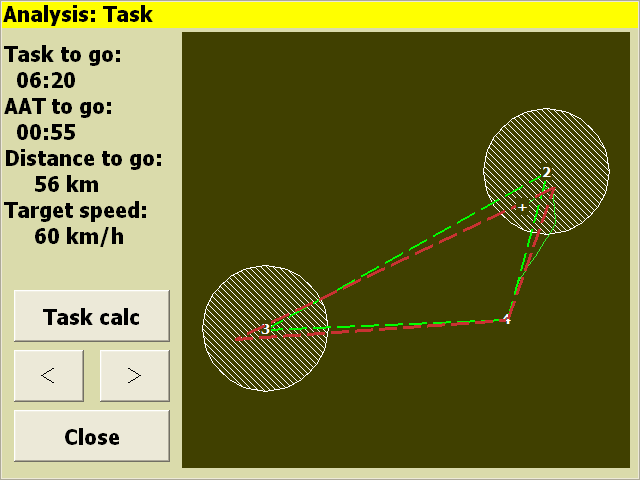
\includegraphics[angle=0,width=0.45\linewidth,keepaspectratio='true']{figures/faat07.png} & 
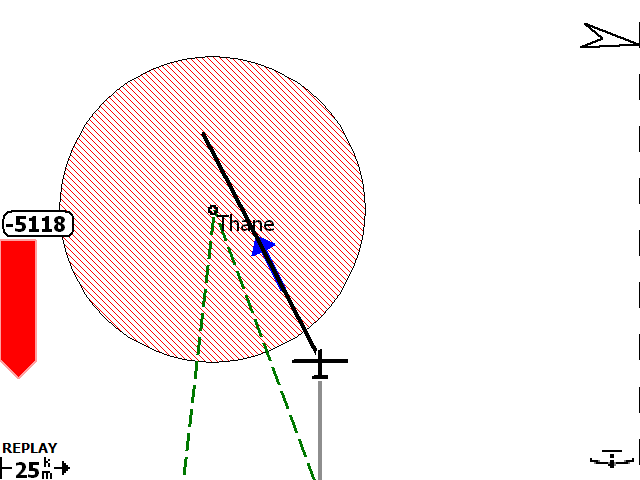
\includegraphics[angle=0,width=0.45\linewidth,keepaspectratio='true']{figures/faat08.png} \\
\emph{Analyses (page circuit)} & \emph{En approche de la prochaine zone} \\
Meilleur objectif calculé & Objectif (60\%) sur la bissectrice \\

\midrule
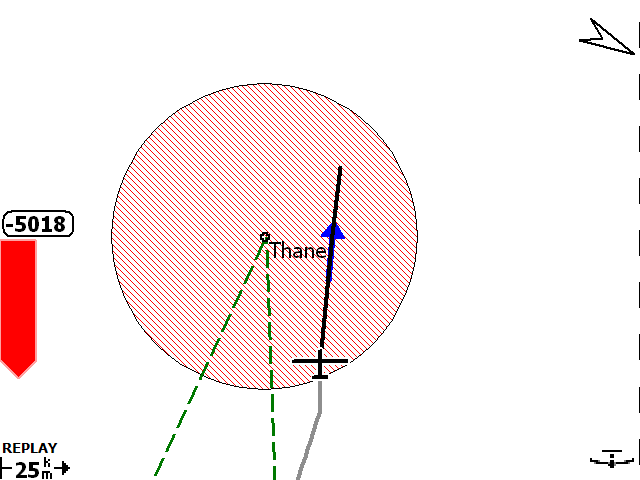
\includegraphics[angle=0,width=0.45\linewidth,keepaspectratio='true']{figures/faat09.png} & 
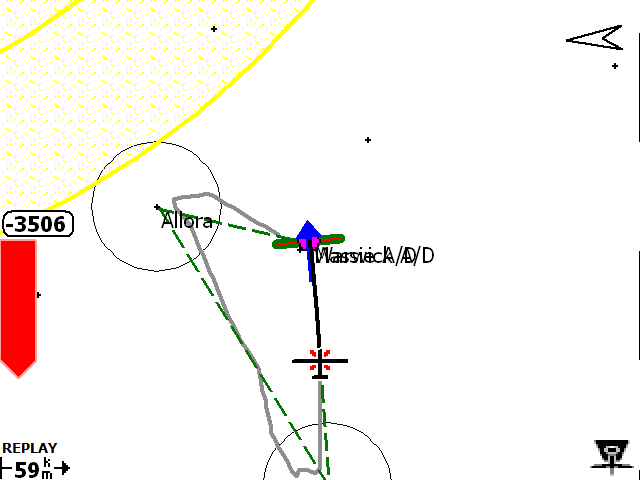
\includegraphics[angle=0,width=0.45\linewidth,keepaspectratio='true']{figures/faat11.png} \\
\emph{Dans la zone} & \emph{Prochain point de virage} \\
Objectif (60\%) projeté sur la route & ``Armer virage'' appuyé \\

\midrule
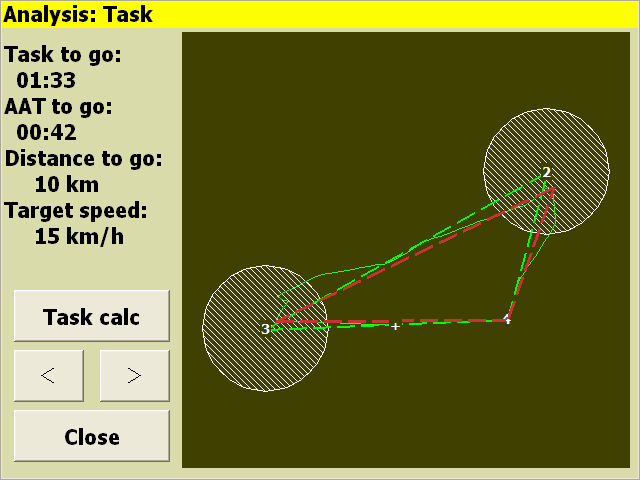
\includegraphics[angle=0,width=0.45\linewidth,keepaspectratio='true']{figures/faat12.png} &  \\
\emph{Analyses (page circuit)} &  \\
Meilleurs objectifs calculés &  \\

\bottomrule
\end{longtable}
\end{center}
\end{maxipage}

\section{OnLine Contest}

La fenêtre d'analyse contient la page ``OLC Plus'' pouvant être
utilisée afin de voir le parcours optimal et le score estimé. Les paramètres de configuration \config{taskrules}
(page des règles de circuit) permettent de choisir l'ensemble des règles à appliquer pour l'optimisation OLC.\@

L'optimisation se fait en permanence en tâche de fond et peut être consultée à volonté. La page d'analyse affiche une vue du parcours
optimisé, la distance et le score. Une InfoBoxe permet aussi d'avoir les valeurs instantanées OLC de distance et de score.

\begin{center}
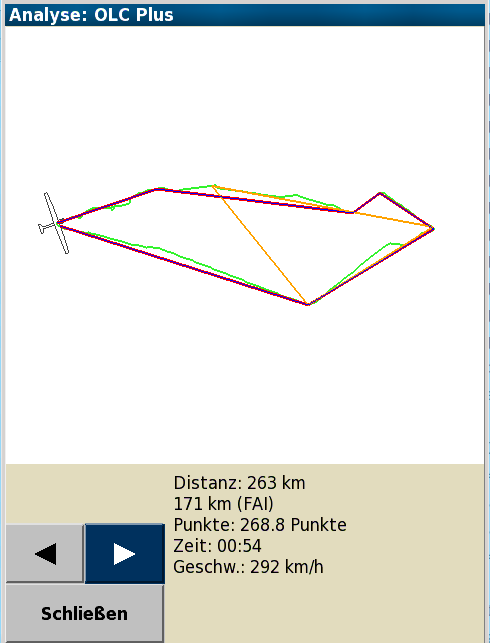
\includegraphics[angle=0,width=0.8\linewidth,keepaspectratio='true']{figures/shot-olc.png}
\end{center}

En vol OLC, les circuits AAT ou non AAT peuvent encore être utilisés pour la navigation. En vol, le calculateur optimise le vol en accord avec les règles OLC choisies.

Dans la page ``Analyses OLC'' la trace du planeur est représentée par une mince ligne verte tandis que le parcours optimal est représenté par une ligne rouge pointillée épaisse.

Le score et la distance optimale calculée sont approximatifs.

Une fois au sol, les résultats ne sont plus mis à jour.


\section{Enregistreur}\label{sec:logger}

Un enregistreur de vol (``logger'') conforme aux règles IGC permet d'enregistrer les vols.

Avec \xc{} on peut accéder à plusieurs enregistreurs~:
\begin{itemize}
\item Un enregistreur basé sur un logiciel. Toutes les versions d'\xc{} proposent cette fonction. L'enregistreur est conforme à la norme IGC mais il n'est pas certifié.
\item \xc{} peut aussi envoyer des déclarations de circuit vers des enregistreurs externes.
Pour que ce soit possible, l'enregistreur doit être sélectionné dans la partie ``Périphériques'' des paramètres de \config{comdevices} configuration.
\item  Pour une partie des nombreux enregistreurs externes, \xc{} peut télécharger des fichiers IGC.\@
Ceci est particulièrement pratique pour les enregistreurs qui ne sont pas facilement démontables du planeur.
\end{itemize}

\subsection*{Configuration}
Pour une matrice complète des fonctionnalités des enregistreurs supportés, voir paragraphe~\ref{sec:supported-varios}.
La configuration est décrite en détails dans le paragraphe~\ref{conf:logger}. Les détails du fichier d'enregistrement se trouvent dans le paragraphe~\ref{sec:logfiles}.

\subsection*{Activation de l'enregistreur}
La mise en route et l'arrêt de l'enregistreur peuvent être manuels ou automatiques. Pour les parapentes,
\xc{} fournit seulement le démarrage automatique. Ainsi, une vitesse
sol faible ou une hauteur faible au-dessus du relief ne stopperont pas l'enregistrement du vol.
Si vous choisissez l'enregistrement automatique ``départ seulement'', il faudra l'arrêter manuellement.
Pour démarrer (ou arrêter) manuellement, utiliser le menu~:
\sketch{figures/logger-startdeclare.png}
\begin{quote}
\bmenug{Config. 3/3}\blink\bmenut{Enregistr.}{Démarrer}
\end{quote}

Quand l'enregistreur interne d'\xc{} est en fonctionnement, un petit ``bouton'' rond vert en 
bas et à droite de la carte clignote une fois par seconde.

Par défaut, \xc{} est configuré en mode de démarrage et arrêt automatiques.
L'enregistrement débute quand \xc{} détecte le début du vol et il s'arrête à l'atterrissage. La confirmation du démarrage
de l'enregistrement avec déclaration n'a lieu qu'en mode manuel. Si
le démarrage est automatique, la déclaration du circuit est aussi automatique.
En mode simulation, l'enregistreur ne peut être démarré automatiquement.

Si un circuit a été déclaré, alors toute tentative de modification du
circuit fait apparaître un message d'avertissement demandant une confirmation
de l'annulation et l'invalidation de la déclaration du circuit. Ceci a pour but de
rendre plus difficile une modification involontaire du circuit qui conduirai à un circuit
déclaré invalide.

L'enregistreur d'\xc, quand il démarre, vérifie s’il y a au moins 500~kO d'espace
libre dans le système de fichiers. S'il y en a moins, \xc{} éliminera
automatiquement les fichiers IGC les plus anciens, jusqu'à disposer de 500~kO. Il n'y a pas de message de confirmation avant d'effectuer cette opération. \warning{}

L'enregistreur interne d'\xc{} met des données dans un tampon mémoire de façon qu'au démarrage
(automatique et manuel) au moins 60~secondes de données antérieures soient enregistrées. Ainsi, la totalité du décollage est correctement
enregistré par \xc. 

\subsection*{Rejouer un enregistrement}\label{sec:logger-replay}
Les vols enregistrés au format IGC par \xc{} ou d'autres enregistreurs peuvent être rejoués. La fenêtre de relecture de l'enregistreur
est accessible par~:
\begin{quote}
\bmenug{Config. 2/3}\blink\bmenug{Rejouer}
\end{quote}
\sketch{figures/loggerreplay.png}

Au cours d'une relecture, le mot ``REPLAY'' s'affiche en bas à gauche de
l'écran et le programme se comporte comme si le GPS  recevait des informations
d'actualisation. La fenêtre de relecture de l'enregistreur n'a pas besoin d'être
ouverte pendant une relecture.

Pour commencer à rejouer un vol, il faut commencer par choisir le fichier à charger, puis appuyer sur
\button{Démarrer}. La vitesse de défilement du vol peut être modifiée en
modifiant le champ ``Taux''. Pour mettre en pause,
mettre la valeur de ``Taux'' à zéro. Des valeurs de taux élevées peuvent conduire à  dégrader
l'estimation du vent et d'autres fonctions de statistiques/analyses.

Pour arrêter de rejouer le vol, appuyer sur \button{Arrêter}.
Lorsqu'un vol est rejoué, le fait de rappuyer sur \button{Démarrer} redémarre
le vol à son début.

\tip{} Quand un fichier de vol a été rejoué, il est recommandé de redémarrer
l'appareil avant de voler, afin de s'assurer que les paramètres de
statistiques internes d'\xc{} soient réinitialisés.

Quand on utilise \xc{} en mode VOL, il n'est pas possible de rejouer un vol
enregistré si le GPS détecte que l'appareil est en mouvement.

La relectur des fichiers de vol fonctionne mieux si l'intervalle entre mesures est inférieur ou égal à 6~secondes.

\subsection*{Enregistreur d'erreur}\label{sec:raw-logger}
Pour la faciliter la recherche de solution à des bugs d'\xc,
il y a un ``enregistreur brut''. Si vous pouvez reproduire un comportement anormal d'\xc, il faut activer cet enregistreur en faisant~:
\begin{quote}
\bmenug{Config. 3}\blink\bmenug{Enregistreur brut}
\end{quote}
Pour corriger un bug, les développeurs apprécieront une description détaillée du problème incluant un fichier de l'enregistreur brut. Celui-ci permet d'accélérer énormément l'analyse de la cause du problème et donc de résoudre l'erreur.

\section{Analyse du vol}\label{sec:analysis-climb}

Les pages d'analyse sont très utiles pour planifier et gérer
les vols sur la campagne. On y accède par le menu~: \gesture{Haut - Droite - Bas}
\begin{quote}
\bmenug{Info. 1/3}\blink\bmenug{Analyses}
\end{quote}

Plusieurs pages sont particulièrement intéressantes~:
\begin{description}
\item[Barographe] Présente un graphique de l'altitude au cours du vol.
Les statistiques sont exploitées pour évaluer la bande de travail en thermique (moyenne
de la base et du sommet des ascendances) et pour estimer la variation de plafond au
cours du temps. La base et le plafond des ascendances sont représentés par des lignes sur le graphe. 

Le bouton \button{Paramètres} ouvre directement la page de configuration des paramètres du vol, permettant de modifier les valeurs des ballast, des moucherons, du QNH et de la température maximum.

\begin{center}
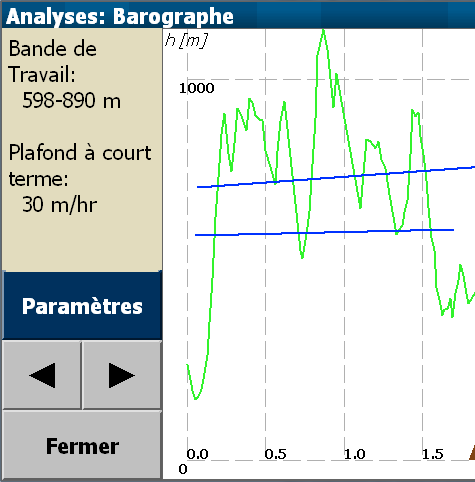
\includegraphics[angle=0,width=0.8\linewidth,keepaspectratio='true']{figures/analysis-barograph.png}
\end{center}

\item[Vario]
Montre sous forme d'un graphique à barres la moyenne de chaque
ascendance. Les statistiques sont utilisées pour calculer la moyenne générale
des ascendances et pour estimer comment cette moyenne évolue au cours du temps. La
valeur actuelle du calage MacCready  est représentée par un tireté rouge
épais, et la tendance du taux de montée par une ligne bleue.

Le bouton \button{Calc.\ circuit} ouvre directement la page principale du gestionnaire de circuit et permet d'ajuster, par exemple, le calage MacCready.

\begin{center}
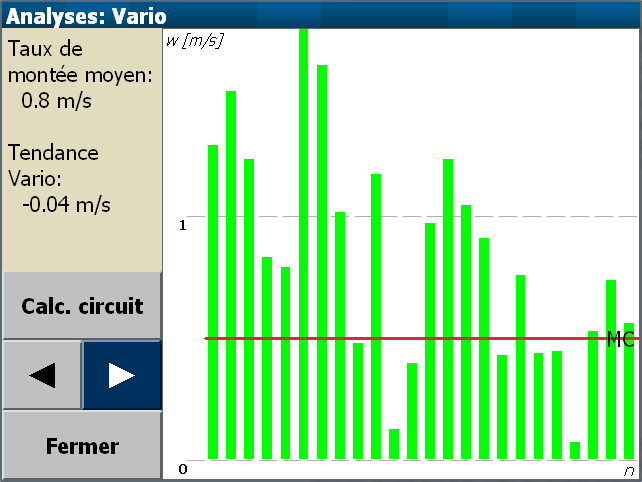
\includegraphics[angle=0,width=0.8\linewidth,keepaspectratio='true']{figures/analysis-climb.png}
\end{center}

\item[Circuit]
Cette page montre le parcours intégral du vol. Le circuit
est représenté par un tireté vert épais, les zones AAT étant ombrées. Pour les circuits
AAT, le chemin restant depuis le planeur jusqu'aux points de virage restants
est en rouge. Le parcours réalisé est représenté par une fine ligne continue verte.

Le bouton \button{Calc.\ circuit} ouvre directement le gestionnaire de circuit et permet de modifier le calage MacCready et la longueur du circuit AAT.\@

\begin{center}
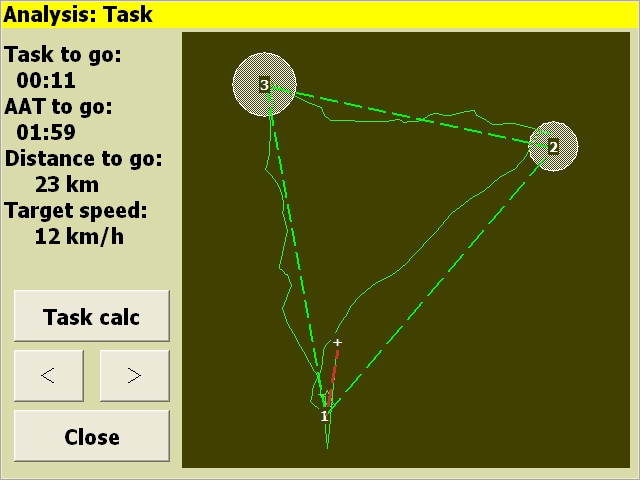
\includegraphics[angle=0,width=0.8\linewidth,keepaspectratio='true']{figures/analysis-task.png}
\end{center}

\end{description}

\section{Heure et levée/coucher de soleil}

L'heure de levée et de coucher du soleil est consultable dans la fenêtre d'états du vol (voir paragraphe~\ref{sec:time-status}). Notez que les conditions atmosphériques locales et l'environnement propre au terrain peuvent conduire à une visibilité très médiocre avant l'heure calculée du coucher de soleil.

Pour les PDA, l'heure d'été est paramétrée par le système d'exploitation du PDA.\@

Si l'heure d'arrivée prévue au dernier point du circuit est après le coucher du soleil, un message d'avertissement est affiché.
